\chapter{Umsetzung}

\section{Gesamt-Architektur}
\begin{itemize}
    \item aktuelles Bild noch entsprechend aufbereiten
    \item sprich BProgram zentral in der Mitte, daneben Simulation-Engines
    \item Logging wird in konkreten Szeanrien genutzt - Visualisierung nutzt Daten aus dem Logger
    \item RL nutzt auch BProgram? -> aktuell noch nicht, aber sollte es eigentlich
\end{itemize}
\begin{figure}[h]
    \centering
    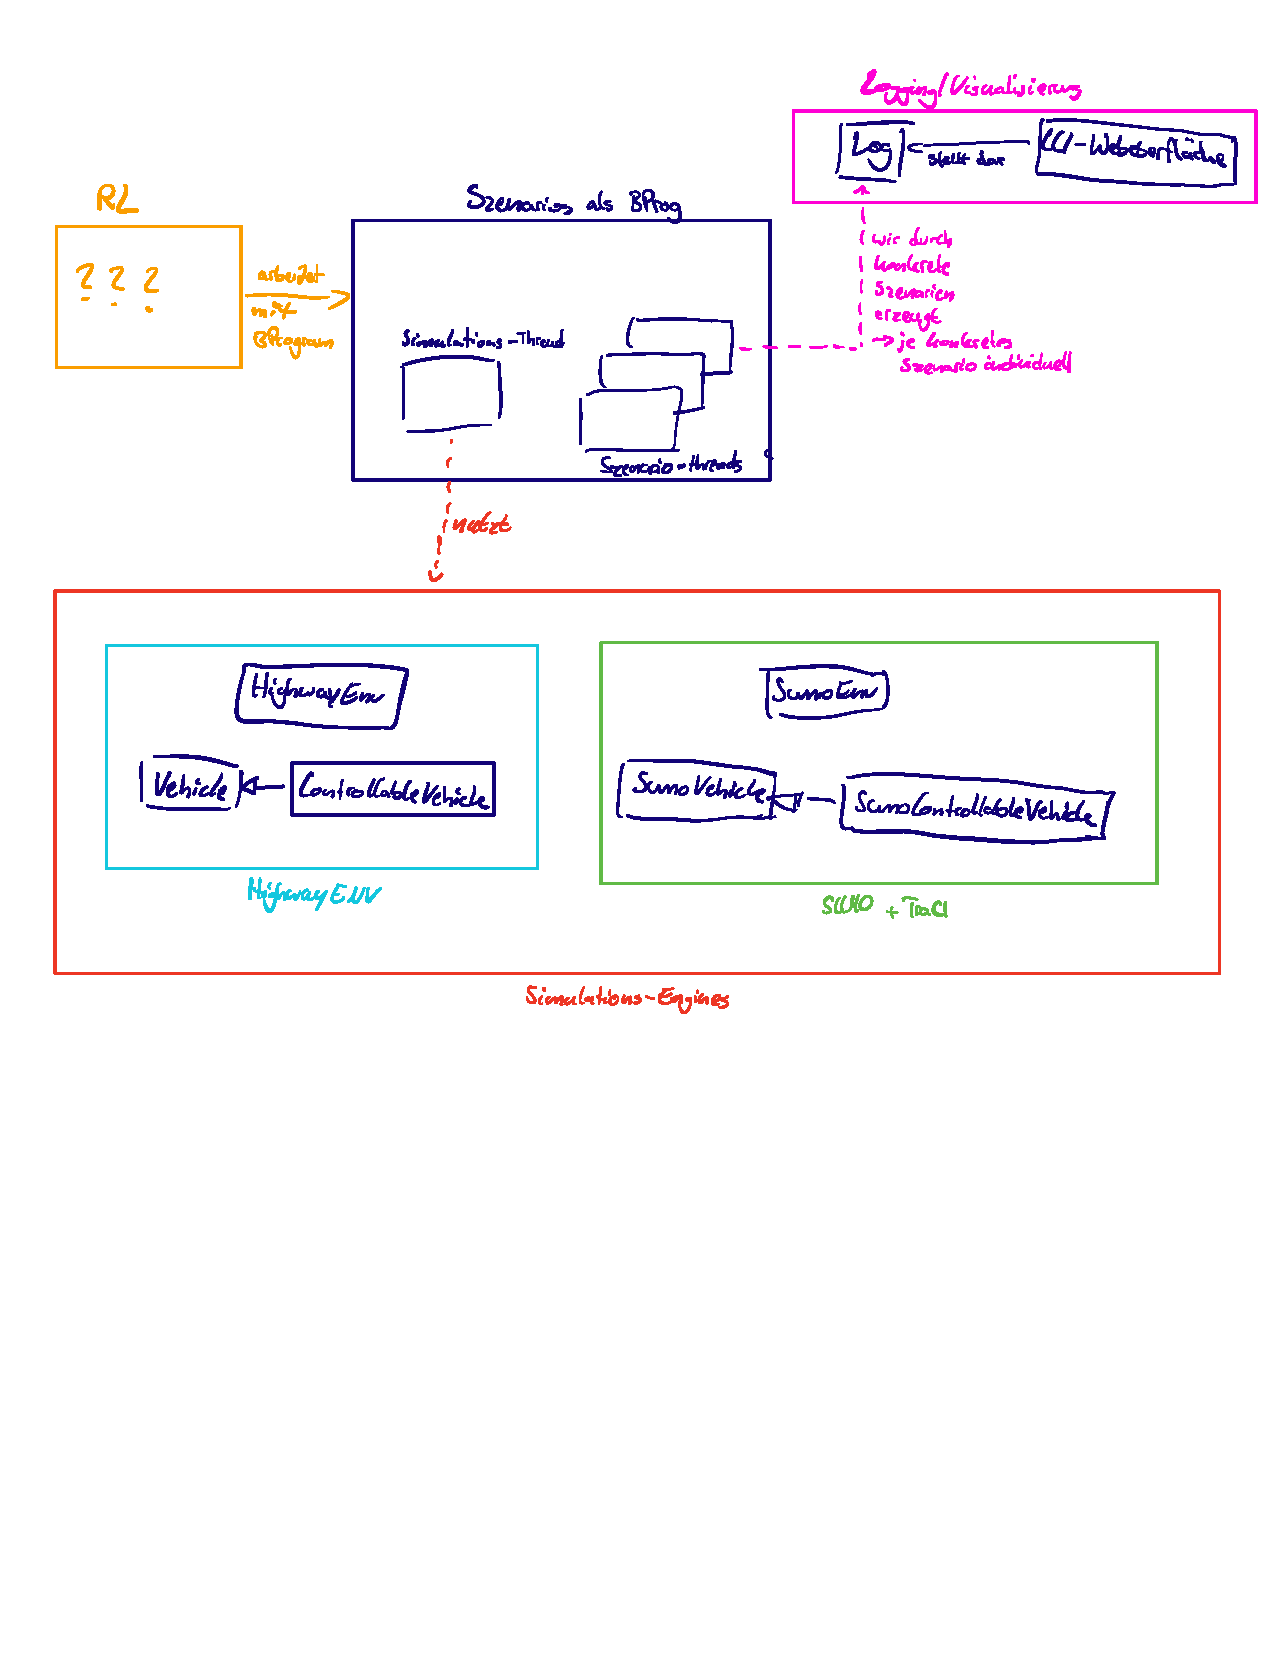
\includegraphics[width=0.8\linewidth]{contents/figures/architecture.pdf}
    \caption{Gesamtarchitekturp}
    \label{fig:architecture}
\end{figure}
\section{Simulationsumgebungen}
\subsection{HighwayEnv}
\subsubsection{Konfiguration von HighwayEnv}
\begin{itemize}
    \item z.B. Multi-Agent-setting
    \item und andere Besonderheiten, die wir in Q1 erarbeitet haben
\end{itemize}
\subsubsection{Integration in das BProgram}
\begin{itemize}
    \item B-Thread für HighwayEnv, wie aufgebaut und warum?
\end{itemize}
\subsubsection{VUT-Ansätze}
\begin{itemize}
    \item Training eines VUT, um es als Testfahrzeug für unsere Testszenarien zu nutzen
\end{itemize}
\subsubsection{Ansätze zum Zugriff auf Fahrzeuginformationen}
\begin{itemize}
    \item Observation-Wrapper-Ansatz
    \item Vehicle-Based Ansatz
    \item Vergleich der beiden Ansätze
\end{itemize}
\subsection{Sumo}
\begin{itemize}
    \item Warum SUMO anstelle von HighwayEnv?
\end{itemize}
\subsubsection{SumoEnv zur Einbindung in das BProgram}
\begin{itemize}
    \item Klasse SumoEnv erklären
    \item implementiert Gym Env-Interface, wie auch HighwayEnv
    \item zur einfacheren Einbindung in unsere bestehende Arbeit
\end{itemize}
\subsubsection{Abbildung der Fahrzeugeigenschaften}
\begin{itemize}
    \item da sich das Vehicle-Konstrukt als praktikabler herausgestellt hat wurde es analog auf Sumo übertragen
    \item somit muss in die bestehenden Szenarien nur die Fahrzeug-Klassen anders instanziiert werden, der Rest bleibt gleich
\end{itemize}
\section{Modellierung von Szenarien mit BPpy}
Für die Modellierung von Szenarien wurde BPpy genutzt. Hierbei wurden verschiedene BThreads erstellt, die unterschiedliche Aspekte der Szenarien abbilden.
Einzelne BThreads bilden bestimmte Funktionalitäten und Teilszenarien ab, die dann in Kombination ein vollständiges, konkretes Szenario ergeben. So können die Funktionalitäten insgesamt besser strukturiert und wiederverwendet werden.
Die BThreads werden aber außer für einzelne Funktionalitäten auch für die Simulation und Abstraktion von Szenarien genutzt, sowie gebündelt um ein konrektes Szenario wie ein Überholmanöver abzubilden.
So gibt es BThreads, die ein abstraktes Szenario modellieren, also die grundlegende Anforderungen an das Szenario definieren, ohne sich auf eine konkrete Implementierung festzulegen. Diese abstrakten Szenarien werden dann im BProgram mit ausgeführt um zu überprüfen, dass die Anforderungen an das Szenario erfüllt werden.
Dabei werden konkrete Angaben überprüft, wie z.B. das sich bestimmte Fahrzeugpositionen verändert haben, oder in welcher Fahrbahn sich die Fahrzeuge im Vergleich zueinander befinden.
Dazu kann dann geloggt werden, ob die Anforderungen erfüllt wurden, und wenn nicht, welche Anforderungen nicht erfüllt wurden.

Der Simulations-Thread hat die Aufgabe, die Simulation zu steuern und sicherzustellen, dass die Szenarien in der Simulationsumgebung korrekt ausgeführt werden. Er sorgt dafür, dass die Fahrzeuge entsprechend den definierten Szenarien agieren und interagieren.
Dabei erhält der Simulations-Thread Informationen von den anderen BThreads, um die Simulation entsprechend anzupassen und zu steuern. Z.B. werden in diesem Thread Aktionen der Fahrzeuge ausgeführt, die von anderen BThreads definiert wurden.
Dieser Thread dient insbesondere der korrekten Übersetzung der Aktionen für die jeweilige Simulationsumgebung, die in diesem Integrationsprojekt entweder HighwayEnv oder Sumo sein kann.
In diesem Thread wird auch auf Kollisionen und andere terminierende Ereignisse geprüft, um die Simulation entsprechend zu beenden oder anzupassen.

Das konkrete Szenario wird durch die Kobination von verschiedenen BThreads modelliert, die zusammen die vollständige Logik und Anforderungen des Szenarios abbilden. Dabei wird spezifische Logik implementiert, die nur für dieses Szenario relevant ist und meist in weitere Methoden ausgelagert.
Die entsprechende Logik wird dann im relevanten BThread aufgerufen, um den Teil des Szenarios zu steuern. Dabei können mehrere BThreads auch zu einem konkreten Szenario gehören, um verschiedene Aspekte abzudecken.
Diese Threads können über ein Paralleitätskonstrukt parallel ausgeführt werden, um die gleichzeitige Ausführung verschiedener Aspekte des Szenarios zu ermöglichen. Spezifische Logik wird in den einzelnen BThreads per \teexttt{yield from} aufgerufen, um diese anzuwenden.
\begin{itemize}
    \item Erklärung der einzelnen BThreads -> Simulation, abstraktes Szenario, konkretes Szenario
    \item am Beispiel von follow-behind-Szenario
\end{itemize}

Die Aufteilung und Aufgaben der einzelnen BThreads wird jetzt noch einmal an einem konkreten Beispiel, dem Follow-Behind-Szenario, erläutert.

\section{Visualisierung von ausgeführten konkreten Szeanrien}
\section{Reinforcement Learning}
Hier wird die Struktur und Funktionalität des Projekts, das ein Reinforcement-Learning-Modell (RL) für Überholszenarien trainiert, speichert und nutzt beschrieben. Die Hauptkomponenten des Projekts sind in mehreren Python-Dateien organisiert.

\texttt{src/envs/overtake\_env.py}
Diese Datei definiert die Umgebung für das Überholszenario, bei dem das VUT zum Überholen des vom Modell gesteuerten Fahrzeugs angeregt werden soll. Sie basiert auf einer Kernumgebung und erweitert diese um spezifische Logik für das Training eines RL-Agenten.
Analog existiert die Datei \texttt{src/envs/intersection\_env.py}, bei dem eine Umgebung für ein Kreuzungsszenario definiert wird.

\begin{itemize}
    \item \texttt{\_\_init\_\_(render\_mode, **config\_overrides)}: Initialisiert die Umgebung mit dem übergebenen Rendermodus. Zusätzlich kann die Konfiguration der Umgebung über den \texttt{config\_overrides} Parameter überschrieben werden.
    \item \texttt{reset(**kwargs)}: Setzt die Umgebung zurück, initialisiert die Position und Geschwindigkeit des Agenten sowie des zu überholenden Fahrzeugs (VUT).
    \item \texttt{step(action)}: Führt einen Schritt in der Umgebung aus, basierend auf der Aktion des Agenten. Berechnet Belohnungen anhand des Zustandes der Simulation, unter anderem der Position der Fahrzeuge im Vergleich zueinander. Abschließen wird überprüft, ob die Episode beendet ist. 
    \item \texttt{render()}: Rendert die Umgebung.
\end{itemize}

\texttt{src/main.py}
Diese Datei enthält den Einstiegspunkt für die Ausführung des Projekts und die Konfiguration der Umgebung.

\begin{itemize}
    \item \texttt{create\_env(config: Dict[str, Any])}: Erstellt eine neue Umgebung basierend auf der übergebenen Konfiguration.
    \item \texttt{set\_config()}: Definiert die Konfiguration der Umgebung, einschließlich Fahrspuren, Fahrzeugpositionen und Beobachtungs-/Aktionsräume.
    \item \texttt{main()}: Führt die Hauptlogik aus, einschließlich der Initialisierung der Umgebung und der Simulation von Aktionen.
\end{itemize}

\texttt{src/training/train\_overtake\_agent.py}
Diese Datei ist für das Training des RL-Modells verantwortlich.

\begin{itemize}
    \item \texttt{make\_env(rank: int)}: Erstellt eine Instanz der Überholumgebung für das Training.
    \item \texttt{RenderCallback}: Eine Callback-Klasse, der die Umgebung während des Trainings in regelmäßigen Abständen rendert. Ihre \texttt{\_on\_step()} Methode wird vom Modell während des Trainings aufgerufen um zu bestimmen ob die aktuelle Episode gerendert werden soll.
    \item \texttt{main()}: Führt das Training des RL-Modells durch. Es initialisiert das Modell und definiert die Traingsumgebung, trainiert es mit der \texttt{DQN}-Methode und speichert das trainierte Modell.
\end{itemize}

\subsection{Trainieren des Modells}
Das Training erfolgt in der Datei \texttt{train\_overtake\_agent.py}. Die Hauptschritte sind:
\begin{enumerate}
    \item Initialisierung der Umgebung mit \texttt{DummyVecEnv}, welchem das zu lernende Szenario übergeben wird.
    \item Definition des RL-Modells mit \texttt{DQN}. Dabei werden diverse Parameter wie der Diskontierungsfaktor für das Lernen des Modells festgelegt.
    \item Start des Trainings mit \texttt{model.learn()}.
\end{enumerate}

\subsection{Speichern des Modells}
Das trainierte Modell wird mit einem Zeitstempel versehen und im Verzeichnis \texttt{models/} gespeichert:
\begin{lstlisting}
model.save("models/overtake_dqn.zip" + current_time)
\end{lstlisting}

\subsection{Nutzen des Modells}
Das gespeicherte Modell kann später geladen und für Inferenz oder weitere Trainingsschritte verwendet werden:
\begin{lstlisting}
from stable_baselines3 import DQN
model = DQN.load("models/overtake_dqn.zip")
\end{lstlisting}